\chapter{Univariate analyse}
\label{ch:analyse1var}

Wanneer onderzoekers een aantal metingen uitgevoerd hebben in een steekproef voor een bepaalde populatie, dan willen we weten welke eigenschappen deze groep als geheel heeft. Het is onpraktisch om alle metingen apart te beschouwen of op te sommen. Om inzichten te krijgen in de verzamelde data, hebben we technieken nodig om deze te visualiseren en samen te vatten. Het geheel van deze technieken wordt \emph{beschrijvende statistiek} genoemd.

\begin{definition}[Beschrijvende statistiek]
  Met beschrijvende statistiek \index{beschrijvende statistiek} bedoelen we een verzameling van technieken om data synthetisch voor te stellen en samen te vatten.
\end{definition}

In dit hoofdstuk gaan we variabelen afzonderlijk beschouwen. In Hoofdstuk \ref{ch:analyse2var} zullen we ook zoeken naar verbanden tussen twee variabelen onderling.

\section{Leerdoelen}
\label{sec:analyse1var-leerdoelen}

Na dit hoofdstuk moet je in staat zijn om:

\begin{itemize}
  \item Voor elk meetniveau de geschikte centrum- en spreidingsmaten te benoemen;
  \item De formules voor gemiddelde, variantie en standaardafwijking van een steekproef te reproduceren en te begrijpen;
  \item Van een gegeven variabele de centrum- en spreidingsmaten te berekenen;
  \item Voor elk meetniveau geschikte visualisatietechnieken te benoemen;
  \item Voor een gegeven variabele geschikte visualisatietechnieken toe te passen;
  \item Een gegeven grafiek te interpreteren, o.a.~het grafiektype benoemen, centrum- en spreidingsmaten afleiden.
\end{itemize}

\section{Centrum- en spreidingsmaten}

Stel je voor dat een groep onderzoekers een studie wil voeren over het verschijnsel superhelden. Vragen die men kan stellen zijn:

\begin{itemize}
  \item Hoe groot zijn superhelden doorgaans?
  \item Hoeveel wegen ze?
  \item Hoe succesvol zijn ze in het veilig maken van hun woonomgeving?
  \item Hoeveel mensen redden ze?
  \item enz.
\end{itemize}

Om de resultaten van metingen samen te vatten, zijn er verschillende methoden en die hangen af van het meetniveau van de betreffende variabele. Enerzijds gaan we op zoek naar een waarde die representatief is voor de hele groep, een \index{centrummaat}\emph{centrummaat}, en anderzijds naar een waarde die aangeeft hoe groot de onderlinge verschillen zijn binnen de groep, een \index{spreidingsmaat}\emph{spreidingsmaat}. Een centrummaat en de bijhorende spreidingsmaat worden vaak als samenvatting gebruikt voor een reeks metingen.

Tabel~\ref{tab:centrum-spreidingsmaten} geeft een overzicht van geschikte centrum- en spreidingsmaten per meetniveau. Deze worden verderop in dit hoofdstuk gedefinieerd.

\begin{table}
  \centering
  \begin{tabular}{lll}
  \toprule
 	\textbf{Meetniveau} & \textbf{Centrummaten} & \textbf{Spreidingsmaten}      \\
  \midrule
 	Kwalitatief         & Modus                 & ---                           \\
  \midrule
 	Kwantitatief        & Gemiddelde            & Variantie, standaardafwijking \\
	                    & Mediaan               & Bereik, interkwartielafstand  \\
  \bottomrule
  \end{tabular}
  \caption[Geschikte centrum- en spreidingsmaten voor elk meetniveau.]{Geschikte centrum- en spreidingsmaten voor elk meetniveau. De centrummaat en bijhorende spreidingsmaat worden vaak gebruikt als samenvatting voor de resultaten van de groep als geheel.}
  \label{tab:centrum-spreidingsmaten}
\end{table}

\section{Kwalitatieve variabelen}

Bij kwalitatieve variabelen is de waarde niet noodzakelijk een getal. De variabele `gender' heeft als waarden onder andere \emph{man} en \emph{vrouw}. Hiermee is het moeilijk te rekenen. Daarom zijn de mogelijkheden om de waarden samenvatten beperkt. Als centrummaat definiëren we de \emph{modus}, maar een bijhorende spreidingsmaat is er niet echt. Om de spreiding over de verschillende voorkomende waarden te tonen, kan je eventueel wel gebruik maken van een frequentietabel die voor elke waarde aangeeft hoe vaak die voorkomt in de dataset.

\subsection{Modus}

\begin{definition}[Modus]
  De \index{modus} modus (Eng. \index{mode}\emph{mode})is de waarde die het meest voorkomt in een verzameling metingen.
\end{definition}

\begin{itemize}
  \item Er kunnen twee modi zijn: in dit geval spreken we van een \index{bimodaal}\emph{bimodale} variabele;
  \item Er kunnen ook meerdere modi zijn: dit noemen we \index{multimodaal} \emph{multimodaal}.
  \item De modus niet veel zin bij een kwantitatieve variabele, waar elke meting typisch uniek is. Soms is het in dat geval nuttig om ze te groeperen in categorieën (zie Voorbeeld~\ref{ex:modale-klasse}).
\end{itemize}

\begin{example}
  \label{ex:modale-klasse}
  De onderzoekers hebben bijgehouden hoeveel mensen Batman elk jaar gered heeft. Hieronder zijn de cijfers voor de laatste negen jaar, onderverdeeld in 4 categorieën.
  
  \begin{itemize}
    \item $[0-9]$ mensen : 4, 7
    \item $[10-19]$ mensen: 11, 16
    \item $[20-29]$ mensen : 20, 22, 25, 26
    \item $[30-39]$ mensen: 33
  \end{itemize}

  Categorie $[20-29]$ komt het meest voor. Dit is de modale klasse. Batman redt dus doorgaans tussen 20 en 29 mensen per jaar.
\end{example}

\section{Kwantitatieve variabelen}

Bij kwantitatieve variabelen is er meer keuze qua centrum- en spreidingsmaten. Voor dit soort variabelen kan je gebruik maken van:

\begin{itemize}
  \item gemiddelde en standaardafwijking;
  \item mediaan en interkwartielafstand.
\end{itemize}

Stel dat de onderzoekers een aantal metingen uitgevoerd hebben van de lengte van superhelden. Je vindt de resultaten in Figuur~\ref{gfx:helden}.

\begin{figure}
  \centering
  \begin{tikzpicture}[xscale=4,yscale=2]
  \draw (0,2) -- (0,0);
  \foreach \num/\label in {0/0, 0.2/20, .4/40, .6/60, .8/80, 1/100, 1.2/120, 1.4/140, 1.6/160, 1.8/180, 2/200}{%
    \draw (0, \num) -- (2.5, \num);
    \draw[shift={(0, \num)}] (1pt,0pt) -- (-1pt,0pt) node[left] {\scriptsize \label};
  }
  
  \node[anchor=north] (hero1) at (0.3,1.5)
  {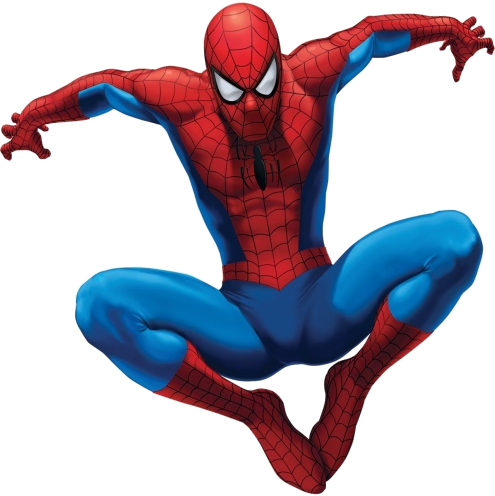
\includegraphics[height=2.9cm]{les2-hero-1}};
  \node[anchor=north] (hero2) at (0.8,2.05)
  {
\includegraphics[height=4cm]{les2-hero-2}};
  \node[anchor=north] (hero3) at (1.3,1.575)
  {
\includegraphics[height=3.1cm]{les2-hero-3}};
  \node[anchor=north] (hero4) at (1.8,2.1)
  {
\includegraphics[height=4.1cm]{les2-hero-4}};
  \node[anchor=north] (hero5) at (2.3,1.95)
  {
\includegraphics[height=3.8cm]{les2-hero-5}};
  
  \node (size1) at (0.3, 1.5) {\scriptsize 141 cm};
  \node (size2) at (0.8, 2.1) {\scriptsize 198 cm};
  \node (size3) at (1.3, 1.51) {\scriptsize 143 cm};
  \node (size4) at (1.8, 2.15) {\scriptsize 201 cm};
  \node (size5) at (2.3, 1.95) {\scriptsize 184 cm};
  \end{tikzpicture}
  \caption{De lengte van enkele superhelden.}
  \label{fig:helden}
\end{figure}

\subsection{Gemiddelde}
\label{sec:gemiddelde}

\begin{definition}[Gemiddelde]
  \index{Gemiddelde} Het rekenkundig gemiddelde (symbool $\overline{x}$, Eng. \index{mean}\emph{mean}, \index{average}\emph{average}) van een verzameling waarden is de som van al deze waarden gedeeld door het aantal waarden.
  \begin{equation}
    \overline{x} = \frac{1}{n} \sum_{i=1}^{n} x_{i}
    \label{eq:Mean}
  \end{equation}

  Waarbij:
  \begin{itemize}
    \item $x_{i}$ de verschillende waarden zijn (in het voorbeeld van Figuur~\ref{fig:helden} zijn dit 141, 198, 143, enz.)
    \item $n$ het aantal waarden is (in het voorbeeld is $n = 5$).
  \end{itemize}
\end{definition}

\begin{remark}[!!]
  Merk op dat we met het symbool $\overline{x}$ specifiek het gemiddelde van een \emph{steekproef} aanduiden. Het gemiddelde van een \emph{populatie} wordt aangeduid met de Griekse letter mu, $\mu$.
  
  Zie Appendix~\ref{app:notatie} voor een overzicht van de gebruikte symbolen en notaties in deze cursus.
\end{remark}

\begin{exercise}
  Wat is de gemiddelde lengte van de superhelden?
\end{exercise}

\begin{exercise}
  Vraag: het gemiddelde van 15 cijfers is 12. Welk nummer moeten
  we aan de rij van cijfers toevoegen om een gemiddelde van 13 te bekomen?
\end{exercise}

\begin{exercise}
  Men zegt dat het rekenkundig gemiddelde gevoelig is aan uitschieters: een extreme waarde kan het rekenkundig gemiddelde zwaar beïnvloeden. 
  
  Stel je voor dat Kabouter Wesley (10 cm) toegevoegd wordt aan het team superhelden. Wat wordt dan de gemiddelde lengte?
\end{exercise}

\subsection{Variantie en standaardafwijking}
\label{sec:varEnSD}

De spreidingsmaat die typisch geassocieerd wordt met het gemiddelde is de standaardafwijking. Voordat we die definiëren, geven we eerst die van de \emph{variantie}.

\begin{definition}[Variantie]
  De \index{variantie} variantie van een steekproef (symbool $s^{2}$, Eng. \index{variance}\emph{sample variance}) is de som van de gekwadrateerde verschillen tussen de waarde van de dataset en het gemiddelde, gedeeld door het aantal waarden min één:
  \begin{equation}
  s^{2} = \frac{1}{n-1} \sum_{i=1}^{n} \left(\overline{x} - x_i \right)^{2}
  \label{eq:variantie}
  \end{equation}
\end{definition}

\begin{example}
  De variantie bij de lengtes van onze superhelden wordt als volgt berekend:
  
  \begin{align*}
  s^{2} &=  \frac{(173,4 - 141)^{2} + (173,4 - 198 )^{2} + (173,4 - 143)^{2} + (173,4 - 201)^{2} + (173,4 - 184 )^{2}}{4} \\
  &=  \frac{(-32,4)^{2} + (24,6)^{2} + (-30,4)^{2} + (27,6)^{2} + (10,6)^{2}}{4}\\
  &= \frac{1049,76 + 605,16 + 924,16 + 761,76 + 112,36}{4}\\
  &= \frac{3453,2}{4} = 863,3
  \end{align*}
\end{example}

Bij de berekening van de steekproefvariantie wordt er gedeeld door $n-1$ en niet door $n$. Waarom? Aangezien de som van de afwijkingen $x_{i} - \overline{x}$ steeds 0 oplevert (zie hieronder in vergelijking \ref{eq:sumGemid}), kan de laatste afwijking gevonden worden uit de eerste $n-1$ afwijkingen. We berekenen dus niet het gemiddelde van $n$ getallen zonder verwantschap. Slecht $n-1$ van de gekwadrateerde afwijkingen kunnen vrij bewegen, daarom berekenen we het gemiddelde door het totaal te delen door $n-1$. Het getal $n-1$ noemt men het aantal \index{vrijheidsgraden}\emph{vrijheidsgraden} van de variantie.

\begin{equation}
 \sum_{i}^{n}(x_{i} - \overline{x}) = \sum_{i}^{n}x_{i} - \sum_{i}^{n}\overline{x} = \sum_{i}^{n}x_{i} - n \left(\frac{1}{n}\sum_{i}^{n} x_{i}\right)
\label{eq:sumGemid}
\end{equation}

\begin{definition}[Standaardafwijking]
  De \index{standaardafwijking} standaardafwijking (Eng. \index{standard deviation}\emph{standard deviation}) wordt dan gedefinieerd als de vierkantswortel van de variantie.
  \begin{equation}
  s = \sqrt{s^{2}} = \sqrt{\frac{1}{n-1} \sum_{i=1}^{n} \left(\overline{x} - x_i \right)^{2}}
  \label{eq:stdev}
  \end{equation}
\end{definition}

\begin{remark}[!!]
  Ook hier hebben we specifiek de variantie en standaardafwijking van een \emph{steekproef} gedefinieerd. De standaardafwijking van een \emph{populatie} wordt aangeduid met de Griekse letter sigma, $\sigma$.
\end{remark}

Dit geeft ons dus inzicht in wat normaal is en wat abnormaal is: een kleine standaardafwijking wijst erop dat de waarden dicht bij de centrummaat ($\overline{x}$) liggen, terwijl een grote standaardafwijking aangeeft dat de waarden verder verspreid liggen. In sommige gevallen wil men een grote standaardafwijking, in andere gevallen niet zoals hieronder beschreven.

\begin{example}
  Bij het vervaardigen van een schroevendraaier is de grootte van de kop belangrijk voor het goed functioneren van de schroevendraaier. Als we dus van 100 verschillende schroevendraaiers de kopgrootte meten, is het beter dat die grootte redelijk constant is en wensen we dus een kleine standaardafwijking.
\end{example}

\begin{example}
  Bij het onderzoek naar onze superhelden, wensen we te weten hoeveel ze ongeveer verdienen in hun normale job. We hebben een aantal rijke superhelden (bv. Batman) en een aantal minder rijke superhelden (bv. Spiderman). De spreiding op hun inkomen is dus groot, maar dat is niet per definitie een probleem.
\end{example}

Een aangename eigenschap van de standaardafwijking is dat het uitgedrukt kan worden in dezelfde metriek als de gemeten data. Bij ons voorbeeld van de superhelden, wil dat zeggen dat de standaardafwijking (ongeveer) 29,38 cm is.

Zoals het gemiddelde zijn de variantie en de standaarddeviatie gevoelig aan uitschieters. De variantie is eigenlijk gevoeliger dan het gemiddelde. Inderdaad, voor een uitschieter is de afstand tot het gemiddelde kleiner dan het kwadraat van deze afstand. % TODO: Wat wordt hiermee bedoeld?

% TODO: Waarom n-1 in de noemer?

\subsection{Mediaan}

De mediaan is een alternatieve centrummaat die als voordeel ten opzichte van het gemiddelde heeft dat die een stuk minder gevoelig is voor uitschieters.

\begin{definition}[Mediaan]
  Indien we alle metingen sorteren van klein naar groot, is de \index{mediaan} mediaan (Eng. \index{median}\emph{median}) het middelste cijfer. Als het aantal cijfers even is, neemt men het gemiddelde van de twee middelste cijfers.
\end{definition}

\begin{exercise}
  Wat is de mediaan van de lengtes van de superhelden?
\end{exercise}

\begin{exercise}
  Wat wordt de mediaan als Kabouter Wesley er bij komt? Is de impact groter of kleiner dan bij het gemiddelde?
\end{exercise}

\subsection{Bereik}

\begin{definition}[Bereik]
  Het \index{bereik}bereik (Eng. \index{range}\emph{range}) van een variabele is de absolute waarde van het verschil tussen de grootste en kleinste waarde.
  \begin{equation}
    | max_i(x_i) - min_i(x_i) |
  \end{equation}
\end{definition}

Het bereik van een variabele is vaak niet zo interessant als spreidingsmaat omdat ze zeer gevoelig is voor uitschieters.

\subsection{Kwartielen \& kwartielafstand}

De interkwartielafstand is een betere spreidingsmaat die veel minder gevoelig is voor uitschieters. Om te begrijpen hoe ze werkt, moeten we eerst het begrip \emph{kwartielen} definiëren.

\begin{definition}[Kwartielen]
  De \index{kwartiel} kwartielen zijn de waarden die een gesorteerde lijst van waarden in 4 gelijke delen deelt. Elk deel vormt dus een kwart van de dataset. Men spreekt van een eerste, tweede en derde kwartiel ($Q_{1}$, $Q_{2}$, $Q_{3}$).
\end{definition}

Dus:

\begin{itemize}
  \item het eerste kwartiel $Q_{1}$ is de waarde die de laagste 25 \% van de reeks afscheidt.
  \item het tweede kwartiel $Q_{2}$ is de waarde die de laagste 50\% van de reeks afscheidt.
  \item het derde kwartiel $Q_{3}$ is de waarde die de laagste 75\% van de reeks afscheidt.
\end{itemize}

Om te bepalen welke waarden in een gesorteerde rij precies de kwartielen zijn, ga je als volgt te werk (volgens \textcite{Moore2002}):

Als $n$ oneven is:

\begin{itemize}
  \item $Q_{1}$ is het $\frac{n+1}{4}$e getal
  \item $Q_{3}$ is het $\frac{3n+3}{4}$e getal
\end{itemize}

Als $n$ even is:

\begin{itemize}
  \item $Q_{1}$ is het $\frac{n+2}{4}$e getal
  \item $Q_{3}$ is het $\frac{3n+2}{4}$e getal
\end{itemize}

\begin{exercise}
  Met welke hiervoor gedefinieerde statistiek komt $Q_{2}$ overeen?
\end{exercise}

\begin{definition}[Interkwartielafstand]
  De \index{interkwartielafstand}interkwartielafstand (Eng. \index{interquartile range}InterQuartile Range, $IQR$) is het verschil tussen het derde en eerste kwartiel.
  
  \begin{equation}
    IQR = Q_3 - Q_1
  \end{equation}
\end{definition}

De definitie van kwartielen kan worden veralgemeend naar \index{deciel}\emph{decielen} (waarden die de dataset in tien gelijke delen verdelen) en \index{percentiel}\emph{percentielen} (honderd gelijke delen). Het 65e percentiel, bijvoorbeeld is dan het getal in de gesorteerde rij waarvoor geldt dat 65\% van de waarden \emph{kleiner} is dan dat getal.

\section{Visualisatie van één variabele}

Ook bij het visualiseren van één variabele hangt het meest geschikte grafiektype af van het meetniveau. In Tabel~\ref{tab:grafiektypes-1-variabele} vind je een overzicht.

\begin{table}
  \centering
  \begin{tabular}{ll}
  	\toprule
  	\textbf{Meetniveau} & \textbf{Grafiektype}          \\
  	\midrule
  	Kwalitatief         & Staafdiagram van frequenties  \\
  	\midrule
  	Kwantitatief        & Boxplot, histogram, dichtheid \\
  	\bottomrule
  \end{tabular}
  \caption{Geschikte grafiektypes per meetniveau voor het visualiseren van één variabele.}
  \label{tab:grafiektypes-1-variabele}
\end{table}

\subsection{Staafdiagram}

Bij het visualiseren van een kwalitatieve variabele wordt eerst een frequentietabel opgesteld van alle voorkomende waarden.

\begin{definition}[Frequentietabel]
  Een \index{frequentietabel}\emph{frequentietabel} is tabel waarin opgesomd staat hoeveel keer een waarde voorkomt in de volledige dataset (= frequentie). Meestal zijn de tabellen verticaal georiënteerd.
\end{definition}

Om de grafiek te tekenen worden de verschillende waarden opgesomd onder de X-as en voor elke waarde wordt een staaf getekend waarvan de hoogte bepaald wordt door het aantal keer dat de overeenkomstige waarde voorkomt.

% TODO: Voorbeeld staafdiagram toevoegen

\subsection{Boxplot}

De \index{boxplot}\emph{boxplot} wordt gevormd door een rechthoek begrensd door de kwartielwaarden (25\% en 75\%). In deze rechthoek wordt ook de mediaan getekend. De stelen, die aan de rechthoek zitten, bevatten de rest van de waarnemingen, op de uitschieters en extremen na.

\begin{itemize}
  \item Een \index{uitschieter}\textit{uitschieter} is een waarde die meer dan 1,5 keer de interkwartielafstand boven/onder het derde/eerste kwartiel ligt en wordt aangeduid met een cirkeltje.
  \item Een \index{extremum}\textit{extremum} is een waarde die meer dan 3 keer de interkwartielafstand boven/onder het derde/eerste kwartiel ligt en wordt in een boxplot aangeduid met een sterretje.
\end{itemize}

Een boxplot wordt horizontaal of verticaal georiënteerd, op basis van wat het duidelijkst is.

% TODO: Voorbeeld boxplot toevoegen

\subsection{Histogram}

Een \index{histogram}\emph{histogram} is een soort staafdiagram, maar dan aangepast naar kwantitatieve variabelen. Het bereik van de variabele wordt onderverdeeld in een door de onderzoeker gekozen aantal, typisch even grote, intervallen. Voor elk interval wordt er geteld hoeveel waarden er binnen vallen en op basis daarvan wordt de hoogte van de staven bepaald.

% TODO: Voorbeeld histogram toevoegen

\subsection{Dichtheidsgrafiek}

% TODO: uitleg en voorbeeld toevoegen

\section{Oefeningen}

\subsection{Centrum- en spreidingsmaten}



\begin{exercise}
  \label{ex:mean-stdev-freq}
  De formules voor steekproefgemiddelde $\overline{x}$ en -variantie $s^2$ staan beschreven in secties \ref{sec:gemiddelde} en \ref{sec:varEnSD}, resp. Hoe moeten we deze formules aanpassen worden om $\overline{x}$ en $s^2$ te berekenen wanneer we te maken hebben met een frequentietabel? Doe dit voor de data in tabel \ref{tab:pinfreq}.
\end{exercise}

\begin{table}
  \centering
  \begin{tabular}{cc}
  	\toprule
  	Pinnen $x$ & Frequentie $f_{x}$ \\
  	\midrule
  	    0      &         2          \\
  	    1      &         1          \\
  	    2      &         2          \\
  	    3      &         0          \\
  	    4      &         2          \\
  	    5      &         4          \\
  	    6      &         9          \\
  	    7      &         11         \\
  	    8      &         13         \\
  	    9      &         8          \\
  	    10     &         8          \\
  	\bottomrule
  \end{tabular}
  \caption{Tijdens het spelen van een kegelspel is bijgehouden hoeveel pinnen telkens omver gegooid werden. Voor elke mogelijke score $x$ is bijgehouden hoeveel keer.}
  \label{tab:pinfreq}
\end{table}

\begin{exercise}
  \label{ex:variance-formula}
  In de formule voor de steekproefvariantie wordt het verschil tussen de meetpunten en het gemiddelde gekwadrateerd. Waarom? Zouden we geen eenvoudiger formule kunnen bedenken die een even goede maatstaf is voor de spreiding van een dataset? Hieronder vind je drie voorstellen (de derde is de ``echte'' formule).

  \begin{align}
    s^{2}_{1} &= \frac{1}{n-1} \sum_{i=1}^{n} (\overline{x} - x) \\
    s^{2}_{2} &= \frac{1}{n-1} \sum_{i=1}^{n} \left| \overline{x} - x\right| \\
    s^{2}_{3} &= \frac{1}{n-1} \sum_{i=1}^{n} (\overline{x} - x)^{2}
  \end{align}

  Pas elke formule toe op de twee datasets hieronder. Door het resultaat te vergelijken zou je moeten kunnen besluiten of de formules geschikt zijn als een spreidingsmaat.
  
  \begin{align*}
    X &= \left\{ 4,4,-4,-4 \right\} \\
    Y &= \left\{ 7,1,-6,-2 \right\}
  \end{align*}

\end{exercise}

\begin{exercise}
Zoek eens zelfstandig op wat de variatieco\"effici\"ent voor een steekproef is. Hoe wordt die gedefinieerd voor een volledige populatie en wat zou je ermee kunnen doen?
\end{exercise}

\begin{exercise}
  \label{ex:ais}
  Beschouw de volgende deelverzameling uit het data frame \texttt{ais} (uit de library DAAG). Bereken voor elk de geschikte centrum- en spreidingsmaten van de variabelen \texttt{sex} en \texttt{ht}.
  
  \begin{enumerate}
    \item de roeiers.
    \item de roeiers, de netballers en de tennissers samen.
    \item de vrouwelijke basketballers en roeiers.
  \end{enumerate}
\end{exercise}

\begin{exercise}
Gebruik de functies \texttt{mean} en \texttt{range} om het gemiddelde en bereik van:
\begin{itemize}
  \item de cijfers 1, 2, \dots, 21 
  \item 50 willekeurige normale waarden, die  worden gegenereerd vanuit een normale distributie met gemiddelde 0 en variantie 1 (functie \texttt{rnorm})
  \item de kolommen \texttt{height} en \texttt{weight} in de data frame \texttt{women} (standaard in R).
\end{itemize}
\end{exercise}

In vorige oefeningen hebben we de verschillende spreidingsmaten en centrummaten besproken. Zoals je merkt worden deze metrieken ook gebruikt in het onderzoek van~\textcite{Akin2016}. In de volgende oefeningen gaan we trachten de resultaten te reproduceren.

Hiervoor hebben we het bestand \texttt{android\_persistence\_cpu.csv} nodig. Je vindt die in de Github-repository van deze cursus, onder directory \texttt{oefeningen/data/oef\_3\_1variabele}

\begin{exercise}
  \label{oef:casus-akin2016-1var}
	Open de file met excel en bekijk de structuur van het document. Hoe ziet die er uit? Kan je de variabelen identificeren en hun type benoemen. 
\end{exercise}

We gaan het programma \texttt{R} gebruiken samen met \texttt{RStudio}. Open de file in \texttt{RStudio}.

\begin{lstlisting}
android_cpu <-  read.csv("android_persistence_cpu.csv", sep=";", dec=",")
attach(android_cpu)
\end{lstlisting}

We hebben nu de data ingeladen. We kunnen eens kijken wat de gemiddelde tijd, de standaarddeviatie, de kwartielen e.a. zijn. Gebruik hiervoor de commando's \texttt{mean}, \texttt{median}, \texttt{quantile}, \texttt{min}, \texttt{max}, \texttt{var}, \texttt{sd}. Je kan ook makkelijk gebruik maken van de methode \texttt{summary}.

\begin{exercise}
	Als je de vorige metrieken berekend hebt, wat kan je daar dan over zeggen. Kan je zinnige conclusies trekken uit de vorige resultaten. Zo ja vermeld ze, zo nee beschrijf waarom je dat denkt.
\end{exercise}

% TODO: Oefening over percentielen toevoegen, bv. gebaseerd op 95th percentile bandwith metering
% https://www.semaphore.com/95th-percentile-bandwidth-metering-explained-and-analyzed/
% http://aboutcolocation.info/95th-percentile-monitoring-explained/

\subsection{Grafieken in R}

% TODO: verwijderen uit de cursus, verplaatsen naar labos

Een histogram is een eenvoudige plot. het toont de frequenties van de data die in een bepaald bereik voorkomen. 

\begin{lstlisting}
hist(android_cpu$Tijd,main="Verdeling van de tijd",xlab="De gemeten cpu tijd");
hist(android_cpu$Tijd,main="Verdeling van de tijd",xlab="De gemeten cpu tijd",breaks=2);
\end{lstlisting}
\begin{exercise}
	Wat concludeer je als je bovenstaande grafiek\footnote{Heb je wat problemen met het genereren van grafieken, volgende link \url{https://www.datacamp.com/community/tutorials/15-questions-about-r-plots\#gs.RK_ORsI} bevat een aantal goede tips and tricks om je op weg te helpen.} genereert? Is dit een zinnig resultaat? Wat gebeurt er als je de variabele breaks verhoogt?
\end{exercise}

Een boxplot toont de mediaan, de kwartielen, het maximum en het minimum van een dataset. Dit geeft ons een duidelijk impressie van hoe de data er uitziet.

\begin{lstlisting}
boxplot(x = android_cpu$Tijd);
boxplot(android_cpu$Tijd,main='Spreiding van de CPU tijd',ylab='Tijd in ms');
\end{lstlisting} 

\begin{exercise}
	De boxplot wordt standaard verticaal getekend. Gebruik het commando \texttt{help(boxplot)} om uit te zoeken hoe we de tekening horizontaal krijgen. 
\end{exercise}

Als je goed geantwoord hebt op de volgende vragen merk je natuurlijk dat het weinig zin heeft de volledige dataset te analyseren, aangezien de dataset verdeeld is over verschillende categorie\"en. We willen dus wel deze statistieken weten, maar per categorie. We kunnen dus een boxplot maken voor elke categorie.

\begin{lstlisting}
boxplot(android_cpu$Tijd~android_cpu$Datahoeveelheid,main='Spreiding van de CPU tijd t.o.v. datahoeveelheid',ylab='Tijd in ms');
\end{lstlisting}

\begin{exercise}
	\label{ex:boxplot}
	Interpreteer de resultaten die je behaalt uit deze grafiek. Zijn deze al wat zinniger?
\end{exercise}

We kunnen hetzelfde doen voor de verschillende soorten dataopslagmogelijkheden in android.

\begin{exercise}
	Zelfde vraag als \ref{ex:boxplot} Interpreteer de resultaten die je behaalt uit deze grafiek. Zijn deze al wat zinniger?
\end{exercise}

We kunnen eens kijken hoe de data eruit ziet over alle categorie\"en heen.

\begin{lstlisting}
boxplot(android_cpu$Tijd~android_cpu$PersistentieType*android_cpu$Datahoeveelheid,main='Spreiding van de CPU tijd',ylab='Tijd in ms');
\end{lstlisting}

Het blijkt dat we wel al een duidelijker zicht krijgen over de data over de categorie\"en heen, maar de figuur is op dit moment te druk. 

We moeten de data dus onderverdelen in categorie\"en namelijk onder \texttt{PersistentieType} en \texttt{Datahoeveelheid}. We gaan hiervoor de functie \texttt{which}\footnote{Je kan ook gebruik maken van de functie \texttt{subset}, wat misschien zelfs eenvoudiger is} gebruiken en kijken hoe de verschillende datahoeveelheden verschillen per datahoeveelheidcategorie. 

\begin{lstlisting}
greenDOA <- android_cpu[which(android_cpu$PersistentieType=='GreenDAO'),];
boxplot(greenDOA$Tijd~greenDOA$Datahoeveelheid);
\end{lstlisting}

\begin{exercise}
  Wat concludeer je uit de vorige grafiek?
\end{exercise}

\begin{exercise}
  Ga nu zelf na welke boxplots er interessant zijn om te maken, en kijken of jouw resultaten overeen met die van \textcite{Akin2016}. Welke conclusies trek je1?
\end{exercise}

\begin{exercise}[Retrieval practice]
  Gebruik de procedure voor retrieval practice uit oefening~\ref{ex:retrieval-practice-meetniveaus} om de \emph{analyse- en visualisatietechnieken voor één variabele} in te studeren.
  
  Geef per meetniveau:
  
  \begin{itemize}
    \item De geschikte centrum- en spreidingsmaten (naam + definities en evt.~formules)
    \item Geschikte grafiektypes
  \end{itemize}
\end{exercise}

\subsection{Antwoorden op geselecteerde oefeningen}

\paragraph{Oefening \ref{ex:mean-stdev-freq}}

\begin{itemize}
  \item $\mu = 7$
  \item $\sigma^2 \approx 5.7333$
  \item $\sigma \approx 2.3944$
\end{itemize}

\paragraph{Oefening \ref{ex:ais}}

Tabel \ref{tab:opl-ais-ht} geeft een overzicht met de belangrijkste centrum- en spreidingsmaten voor de variabele \texttt{ht} (height, lengte) over de gevraagde groepen.

\begin{table}
  \centering
  \begin{tabular}{@{}l|r|rrrr|rr@{}}
    \toprule
    & \textbf{(1)} & \multicolumn{4}{c}{\textbf{(2)}}                                                 & \multicolumn{2}{c}{\textbf{(3)}} \\ 
    & \textbf{Row} & \textbf{hele groep} & \textbf{Row} & \textbf{Netball} & \textbf{Tennis} & \textbf{B\_ball}  & \textbf{Row} \\ \midrule
    \textbf{gemiddelde} & 182.376      & 179.066                      & 182.376      & 176.087          & 174.164         & 182.269           & 178.859      \\
    \textbf{stdev}      & 7.798        & 7.936                        & 7.798        & 4.124            & 9.858           & 8.621             & 5.970        \\
    \textbf{min}        & 156.000      & 156.000                      & 156.000      & 168.600          & 157.900         & 169.100           & 156.000      \\
    \textbf{Q1}         & 179.300      & 174.200                      & 179.300      & 173.450          & 167.300         & 174.000           & 177.600      \\
    \textbf{mediaan}    & 181.800      & 179.500                      & 181.800      & 176.000          & 175.000         & 184.600           & 179.650      \\
    \textbf{Q3}         & 186.300      & 183.400                      & 186.300      & 179.150          & 180.750         & 188.700           & 181.200      \\
    \textbf{max}        & 198.000      & 198.000                      & 198.000      & 183.300          & 190.800         & 195.900           & 186.300      \\
    \textbf{IQR}        & 7.000        & 9.150                        & 7.000        & 5.700            & 13.450          & 14.700            & 3.600        \\ \bottomrule
  \end{tabular}
  \caption{Overzicht resultaten in oefening \ref{ex:ais} voor de variabele \texttt{ht} (height/lengte), met drie cijfers na de komma. In deeloefening 2 zijn de resultaten zowel gegeven voor de hele groep (roeiers, netballers én tennissers) als opgesplitst (via de functie \texttt{aggregate}).}
  \label{tab:opl-ais-ht}
\end{table}

In deeloefening 1 en 2 nemen we de variabele \texttt{sex} als voorbeeld. Zie tabel \ref{tab:opl-ais-sex} voor een overzicht. Over kwalitatieve variabelen valt minder te zeggen, we geven hier een frequentietabel waaruit we de modus kunnen afleiden.

In deeloefening 3 zijn enkel vrouwen geselecteerd, en voor deze oefening tonen we in tabel \ref{tab:opl-ais-sport} de frequenties van variabele \texttt{sport}.

\begin{table}
  \centering
  \begin{tabular}{@{}l|r|rrrr}
  	\toprule
  	               & \textbf{(1)} &                    \multicolumn{4}{c}{\textbf{(2)}}                     \\
  	               & \textbf{Row} & \textbf{hele groep} & \textbf{Row} & \textbf{Netball} & \textbf{Tennis} \\ \midrule
  	\textbf{f}     &           22 &                  52 &           22 &               23 &               7 \\
  	\textbf{m}     &           15 &                  19 &           15 &                0 &               4 \\
  	\textbf{modus} &            f &                   f &            f &                f &               f \\ \bottomrule
  \end{tabular}
  \caption{Overzicht resultaten in oefening \ref{ex:ais} (1) en (2) voor de variabele \texttt{sex}. Meer bepaald zijn hier de frequenties van de waarden opgegeven, en ook telkens de modus.}
  \label{tab:opl-ais-sex}
\end{table}

\begin{table}
  \centering
  \begin{tabular}{@{}l|l}
  	\toprule
  	                 & Frequenties \\ \midrule
  	\textbf{B\_ball} & 13          \\
  	\textbf{Row}     & 22          \\
  	\textbf{modus}   & Row         \\ \bottomrule
  \end{tabular}
  \caption{Overzicht resultaten in oefening \ref{ex:ais} (3) voor de variabele \texttt{sport}.}
  \label{tab:opl-ais-sport}
\end{table}